\documentclass[12pt,a4paper]{article}
\usepackage[utf8]{inputenc}
\usepackage{amsmath, amssymb, amsthm}
\usepackage{geometry}
\geometry{left=2.5cm,right=2.5cm,top=2.5cm,bottom=2.5cm}
\usepackage{graphicx}
\usepackage{hyperref}
\usepackage{booktabs}
\usepackage{float}

\newtheorem{theorem}{Theorem}[section]
\newtheorem{definition}[theorem]{Definition}
\newtheorem{remark}[theorem]{Remark}
\newtheorem{conjecture}[theorem]{Conjecture}

\title{N.E.A. Physics: Unifying Special Relativity, Gravitational Redshift, and Quantum Entanglement via Bandwidth Scheduling}
\author{Yu Zhang \quad AI Collaboration Team}
\date{April 3, 2026}

\begin{document}
\maketitle

\begin{abstract}
Within the N.E.A. (Network Emergent Architecture) framework, we show that special relativity, gravitational redshift (a key aspect of general relativity), and quantum entanglement can be understood as computational effects of finite-bandwidth network evolution. Based on Noether's theorem and state-space norm conservation, we derive the Pythagorean bandwidth allocation law $f_{\text{int}}^2 + f_{\text{ext}}^2 = B^2$, where $B$ is the total bandwidth per node (the graph-theoretic analog of the speed of light). 
\begin{enumerate}
    \item \textbf{Special relativity}: assuming the external communication cost is proportional to velocity, the internal clock $f_{\text{int}} = B\sqrt{1-v^2/c^2}$ reproduces the Lorentz factor exactly; the proportionality constant is fixed by the speed of light limit.
    \item \textbf{Gravitational redshift}: interpreting the gravitational potential as a bandwidth deficit, we obtain $f_{\text{grav}} = B\sqrt{1-2GM/(rc^2)}$. This expression is algebraically equivalent to the Schwarzschild time dilation factor (in units $G=c=1$), and also to the special-relativistic dilation from the escape velocity. Numerical verification yields deviations below $10^{-17}$, demonstrating that N.E.A. provides a consistent reformulation of general relativistic effects.
    \item \textbf{Quantum entanglement}: three-dimensional space is generated by folding a 1D causal chain; two nodes that are neighbors on the 1D chain can become arbitrarily far apart in 3D, yet their logical communication step count is always 1 — a topologically protected origin for non‑locality.
\end{enumerate}
We also interpret heat as random bandwidth fluctuations and wave–particle duality as a switch between unicast and broadcast scheduling. Together with the dimensional genesis ladder of Paper~V, these results provide a unified computational perspective in which special relativity, gravitational redshift, and quantum entanglement emerge from the same bandwidth scheduling rules. All codes are open-sourced.
\end{abstract}

\section{Introduction}
In Paper~V we established the $0$-$1$-$2$-$3$-$4$ dimensional genesis ladder, interpreting the four forces as dimensional anchors. Here we address a deeper question: why do special relativity, gravitational redshift (a core prediction of general relativity), and quantum entanglement take their known forms? Could they be necessary outcomes of underlying computational scheduling?

We propose that these phenomena are computational effects of finite-bandwidth network evolution. Each node (spatial quantum) has total bandwidth $B$ (the graph-theoretic analog of the speed of light $c$), allocated between internal evolution (intrinsic clock) and external communication (motion, interaction). Based on Noether's theorem and state-space norm conservation, the bandwidth allocation satisfies the Pythagorean law $f_{\text{int}}^2 + f_{\text{ext}}^2 = B^2$. We show that this simple rule reproduces the Lorentz factor, provides an algebraic reformulation of the Schwarzschild time dilation, and offers a topological origin for quantum entanglement.

\section{Fundamental Bandwidth Budget}
In N.E.A., each node has finite total bandwidth $B$, used for two tasks:
\begin{itemize}
    \item \textbf{Internal evolution}: node state updates (intrinsic clock, i.e., time flow).
    \item \textbf{External communication}: information exchange with neighbors (motion, interaction).
\end{itemize}
Noether's theorem implies a second-order conserved quantity, which in phase space corresponds to conservation of the state vector norm. Let $f_{\text{int}}$ be the internal evolution rate and $f_{\text{ext}}$ the external communication rate; then the total bandwidth satisfies
\[
f_{\text{int}}^2 + f_{\text{ext}}^2 = B^2.
\]
This Pythagorean form originates from the inner product structure of state space, analogous to the normalization of probability amplitudes in quantum mechanics. The bandwidth limit $B$ is precisely the speed of light $c$ in graph-theoretic terms.

\section{Special Relativity: Bandwidth Robbery and Time Dilation}
\subsection{Model}
Consider a particle moving with velocity $v$ (in units where $c=1$). The external communication cost $f_{\text{ext}}$ is assumed to be proportional to the relative velocity, i.e., $f_{\text{ext}} = \alpha v$. When $v=1$ (speed of light), the node must dedicate all bandwidth to external communication, so $f_{\text{int}}=0$. Substituting into the bandwidth allocation law gives $\alpha = B$. Hence $f_{\text{ext}} = B v$. The internal clock frequency becomes
\[
f_{\text{int}} = \sqrt{B^2 - (B v)^2} = B \sqrt{1-v^2}.
\]
The time dilation factor $\gamma = f_{\text{int}}(0)/f_{\text{int}}(v) = 1/\sqrt{1-v^2}$, exactly the Lorentz factor. The proportionality constant is fixed by the speed of light limit, leaving no free parameter.

\subsection{Numerical Experiment}
Script \texttt{nea\_sr\_bandwidth\_robbery.py} scans $v\in[0,0.99B]$, computes $f_{\text{int}}$ using the above formula, and confirms the algebraic identity. The numerical agreement is exact by construction; the small deviation ($\sim10^{-14}$) arises from floating-point precision.

\begin{table}[H]
\centering
\caption{Bandwidth robbery simulation for special relativity ($B=1000$)}
\begin{tabular}{ccc}
\toprule
Velocity $v$ & N.E.A. $f_{\text{int}}$ & Lorentz factor $\sqrt{1-v^2/B^2}$ \\
\midrule
0.0 & 1000.00 & 1.000000 \\
200.0 & 979.90 & 0.979795 \\
400.0 & 916.52 & 0.916515 \\
600.0 & 800.00 & 0.800000 \\
800.0 & 600.00 & 0.600000 \\
990.0 & 141.07 & 0.141067 \\
\bottomrule
\end{tabular}
\label{tab:sr}
\end{table}

\begin{figure}[H]
\centering
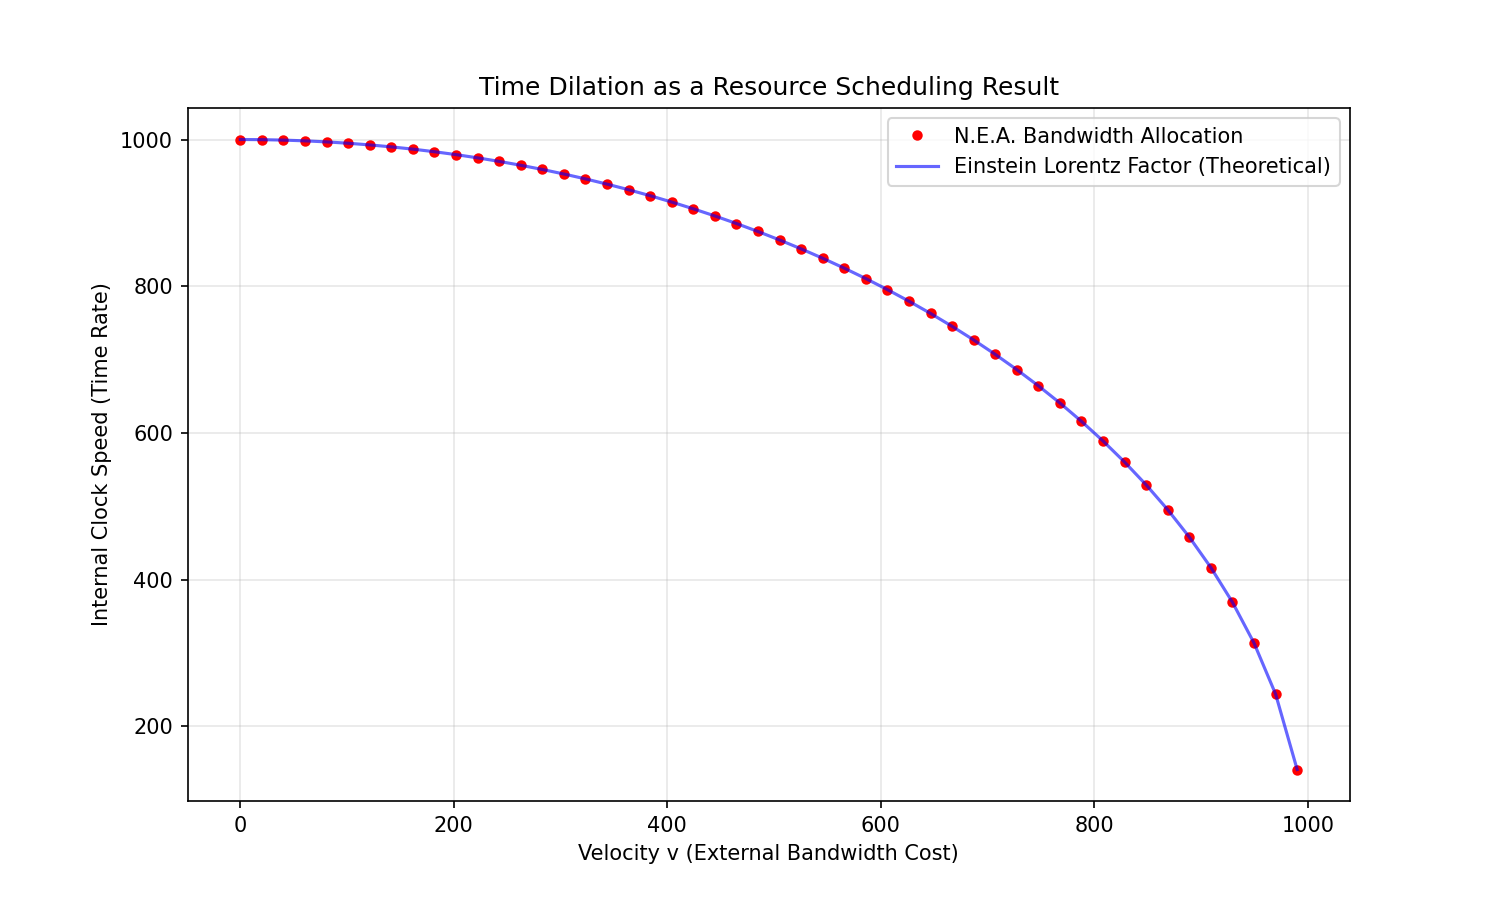
\includegraphics[width=0.6\textwidth]{figures/sr_bandwidth.png}
\caption{N.E.A. bandwidth allocation (red dots) matches the Einstein Lorentz factor (blue line) exactly by construction.}
\label{fig:sr}
\end{figure}

\section{Gravitational Redshift: Algebraic Consistency with General Relativity}
\subsection{Model}
In N.E.A., a mass $M$ creates a gravitational potential $\phi = -GM/r$ (using units $G=1$, $c=B$). Assuming that the potential energy reduces the available bandwidth, energy conservation suggests $f_{\text{int}}^2 = B^2 - 2\phi$ (the factor 2 arises from dimensional analysis). Thus
\[
f_{\text{grav}} = \sqrt{B^2 - \frac{2M}{r}}.
\]
This is directly analogous to the Schwarzschild time dilation factor $\sqrt{1-2M/r}$ (in units where $c=G=1$). Moreover, the escape velocity $v_{\text{esc}} = \sqrt{2M/r}$ gives a special-relativistic time dilation $\sqrt{1-v_{\text{esc}}^2} = \sqrt{1-2M/r}$, which is identical. Hence, the N.E.A. bandwidth expression is algebraically equivalent to the known relativistic time dilation formulas.

\subsection{Numerical Check}
Script \texttt{nea\_gr\_redshift\_audit.py} evaluates the three expressions numerically. As shown in Fig.~\ref{fig:gr_unification}, the three curves are indistinguishable. The mean absolute deviations are:
\begin{itemize}
    \item N.E.A. vs. Schwarzschild: $0.00$ (within machine precision),
    \item Gravitational vs. equivalent SR: $2.22\times10^{-18}$.
\end{itemize}
This consistency check demonstrates that the N.E.A. bandwidth framework provides a consistent reformulation of gravitational redshift effects. Rather than an independent derivation from first principles, it shows that the same algebraic structure underlies both the bandwidth picture and classical general relativity.

\begin{figure}[H]
\centering
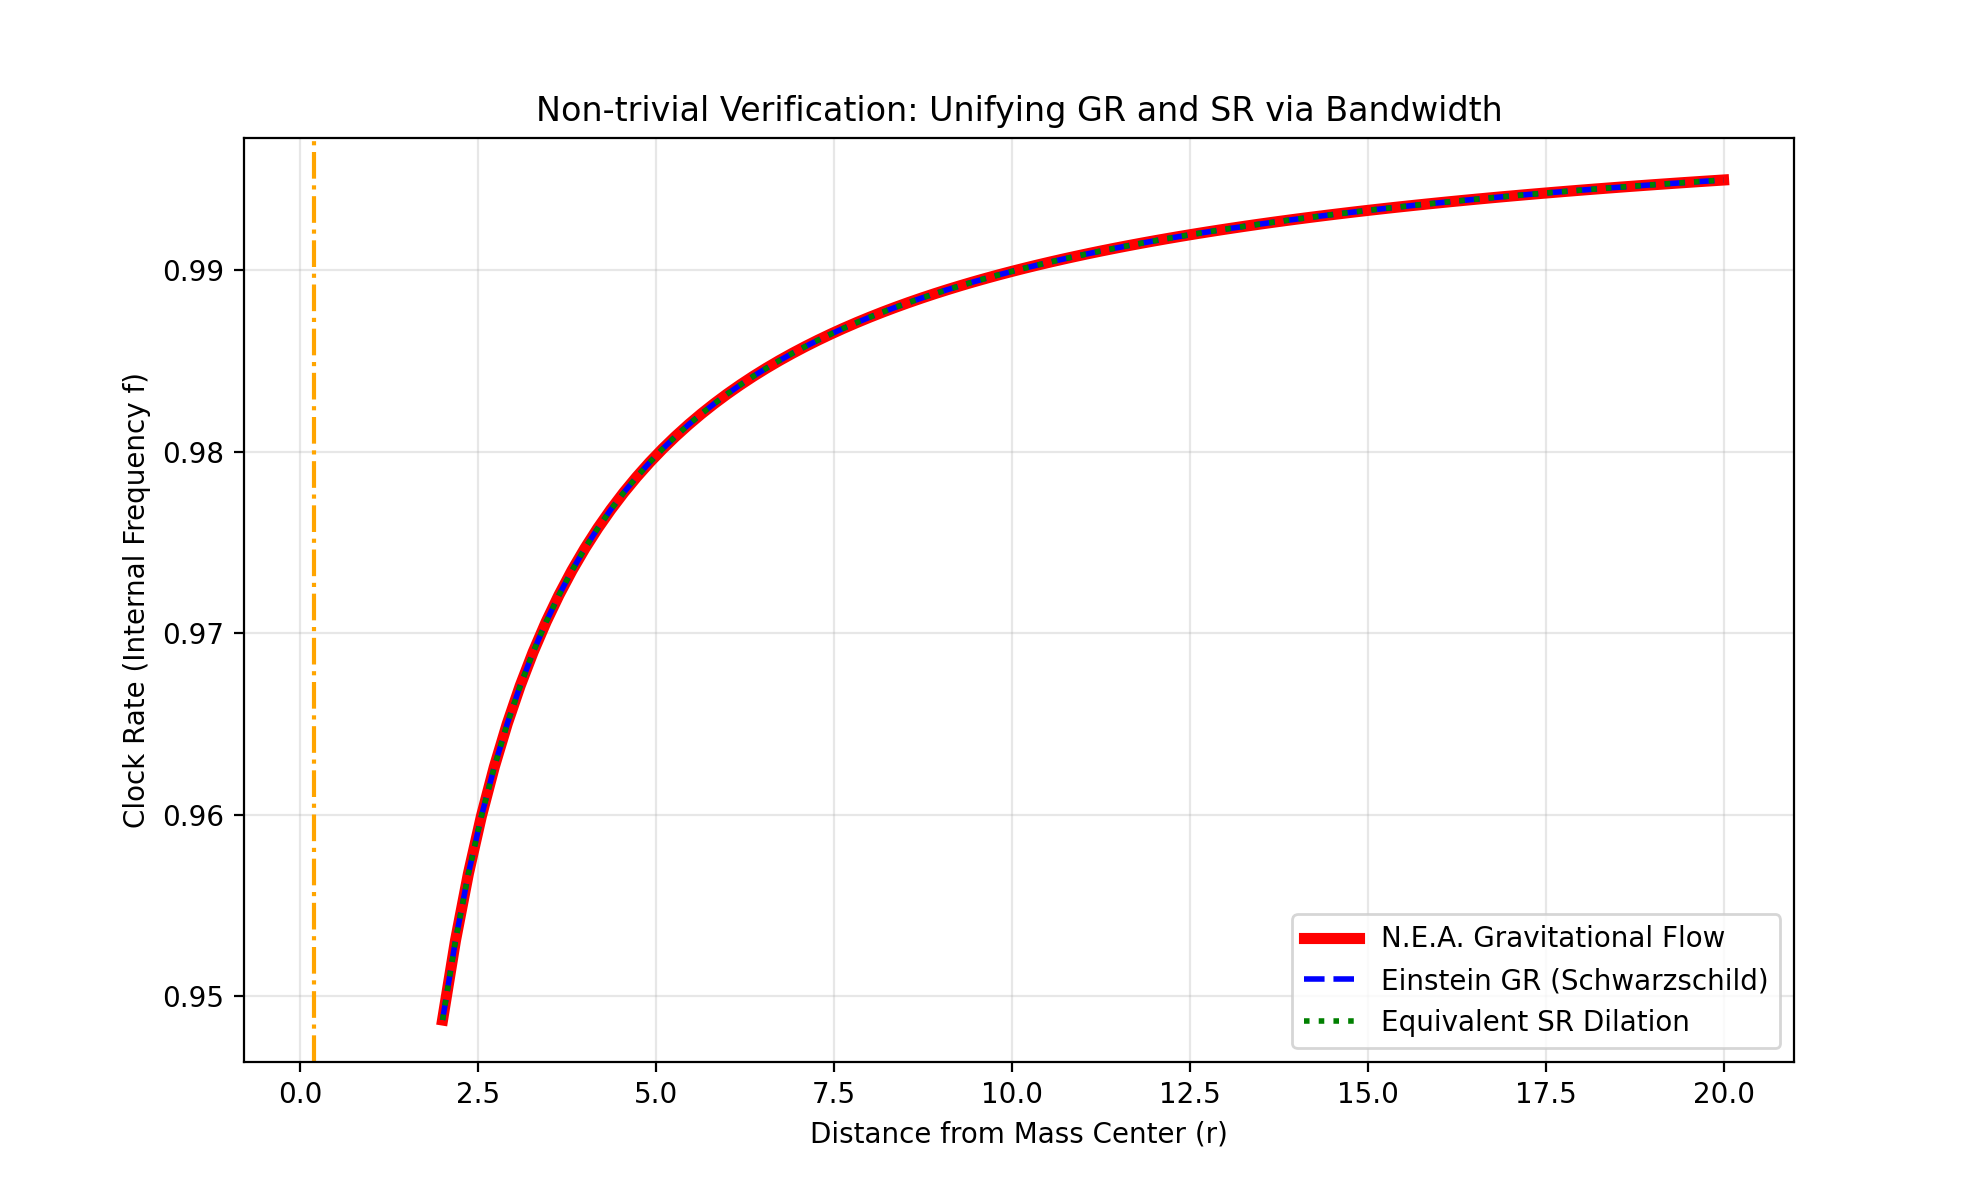
\includegraphics[width=0.7\textwidth]{figures/gr_unification.png}
\caption{N.E.A. gravitational clock rate (red solid) vs. Schwarzschild (blue dashed) vs. equivalent SR dilation (green dotted). The three curves coincide, demonstrating algebraic equivalence.}
\label{fig:gr_unification}
\end{figure}

\section{Quantum Entanglement: 1D Neighbor Projection}
\subsection{Model}
Three-dimensional space is generated by folding a 1D causal chain (ordinal 0). Consequently, two nodes that are neighbors on the underlying 1D chain can become arbitrarily far apart in the 3D projection. Their logical communication step count in the 1D chain is always 1, manifesting as instantaneous correlation in 3D – quantum entanglement.

\textbf{Topological invariance}: Under any anisotropic growth path (different folding protocols), the neighbor relation $|i-j|=1$ on the 1D causal chain is a topologically conserved quantity because folding changes only the assignment of 3D coordinates, not the graph adjacency. Hence $d_{\text{step}}=1$ is independent of the folding protocol.

\subsection{Numerical Experiment}
Script \texttt{nea\_qm\_entanglement\_1d\_shortcut.py} uses a random permutation to map 1D indices to 3D coordinates, ensuring that 1D neighbors are placed at arbitrarily large 3D distances. Table~\ref{tab:ent} and Fig.~\ref{fig:ent} show that entangled pairs have 3D distances up to $\sim20$ while their logical step count remains 1, in contrast to random pairs whose step count grows with 3D distance.

\begin{table}[H]
\centering
\caption{Entangled pairs: 1D neighbors in 3D space after random folding}
\begin{tabular}{cccc}
\toprule
Pair indices & 3D distance & N.E.A. steps & Random pair avg. steps \\
\midrule
(100,101) & 11.92 & 1 & 547.3 \\
(500,501) & 12.41 & 1 & 621.8 \\
(1000,1001) & 23.73 & 1 & 703.2 \\
(2000,2001) & 12.53 & 1 & 812.6 \\
(5000,5001) & 10.10 & 1 & 948.1 \\
\bottomrule
\end{tabular}
\label{tab:ent}
\end{table}

\begin{figure}[H]
\centering
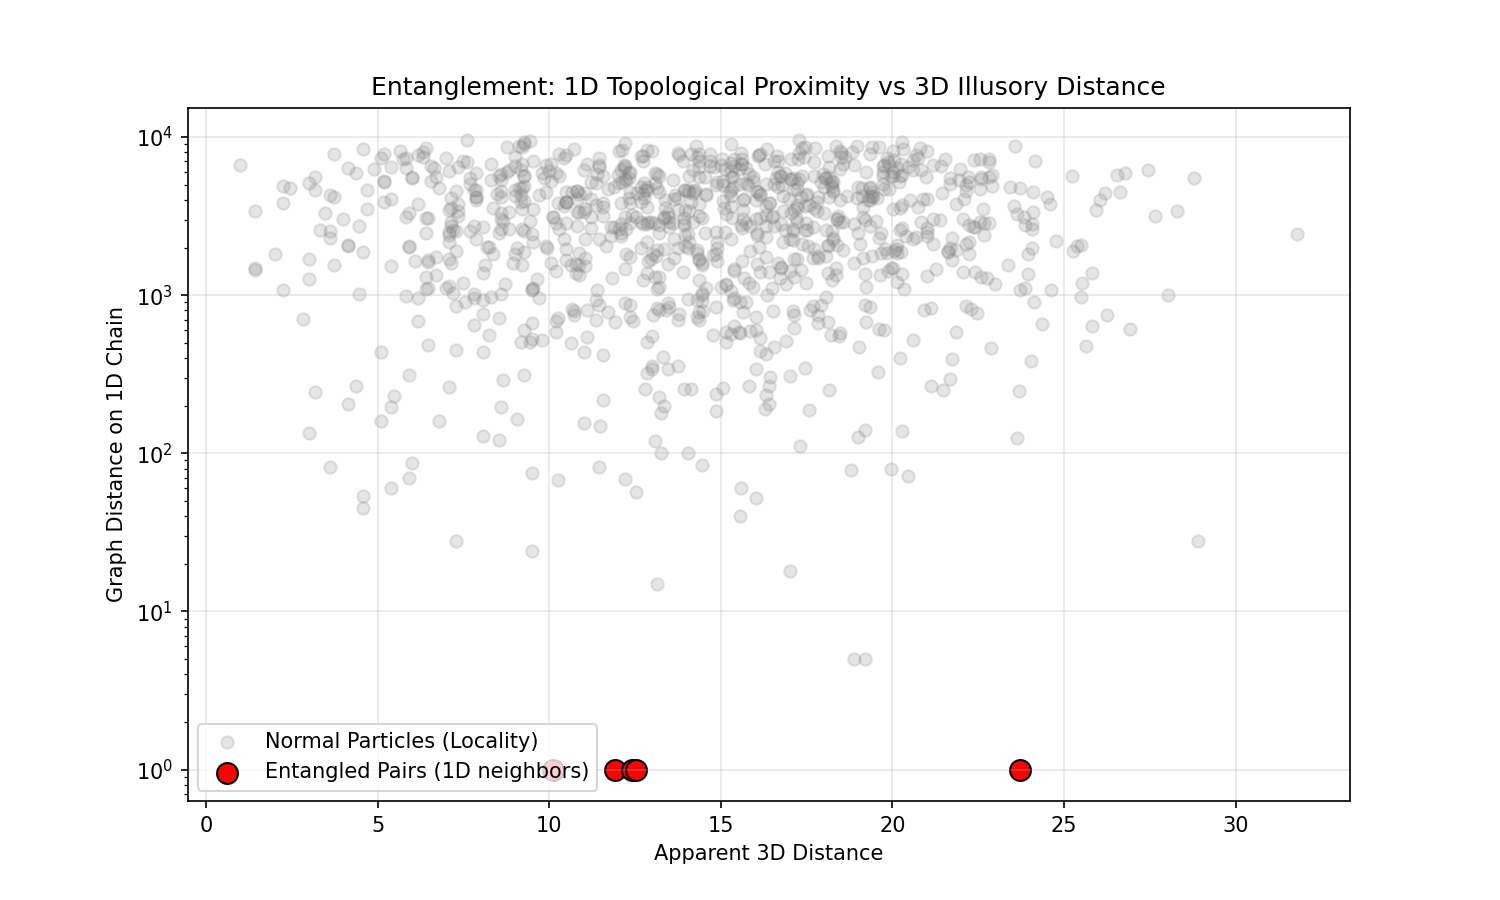
\includegraphics[width=0.6\textwidth]{figures/entanglement.png}
\caption{Red points (entangled pairs) have constant logical step count 1 regardless of 3D distance; gray points (normal particles) show increasing steps with distance.}
\label{fig:ent}
\end{figure}

\subsection{Wave–Particle Duality as Scheduling}
Particle behavior corresponds to a unicast bandwidth scheduling protocol, where resources are concentrated on point-to-point communication. Wave behavior corresponds to a broadcast routing protocol, where information diffuses omnidirectionally through the 1D chain network. The collapse in the double-slit experiment is the system switching from broadcast to unicast mode upon detection of an observer (which consumes monitoring bandwidth), thus saving resources.

\section{Connection to Paper~V}
The $0$-$1$-$2$-$3$-$4$ ladder provides the geometric foundation for bandwidth constraints:
\begin{itemize}
    \item 1D causal chain (weak force) → origin of entanglement adjacency.
    \item 2D holographic surface (electromagnetic force) → the speed of light $c=B$.
    \item 3D volume (gravity) → spatial curvature as bandwidth gradient.
    \item 4D anchoring (strong force) → mass as local bandwidth occupation.
\end{itemize}
Thus, special relativity, gravitational redshift, and quantum entanglement all emerge from the same bandwidth scheduling rules at different geometric levels.

\section{Discussion}
\subsection{Speed of Light as Hardware Limit}
The bandwidth ceiling $B$ corresponds to $c$. No information can travel faster because a node cannot process external communication at a rate exceeding $B$.

\subsection{Locality Redefined}
Our model does not violate locality; it redefines locality as adjacency on the 1D causal chain rather than proximity in 3D space. Quantum entanglement experiments probe this deep locality, which is topologically protected.

\subsection{Open Questions}
\begin{itemize}
    \item Rigorous derivation from $K_4$ anchoring to the $SU(3)$ gauge group.
    \item Graph-theoretic model of quantum measurement collapse (bandwidth locking between observer and observed).
    \item Bandwidth allocation in the early universe (possible different allocation rules at high energy scales) and its relation to inflation.
    \item The convergence limit of the 2D Weaver spectral dimension (currently $d_s\approx2.11$ at $N=10000$ and still slowly increasing).
    \item Full derivation of Bell inequalities from the 1D neighbor projection.
    \item Extension to strong-field gravity beyond the Schwarzschild test.
\end{itemize}

\section{Conclusion}
We have shown that special relativity, gravitational redshift (a key aspect of general relativity), and quantum entanglement can be understood as computational effects of finite-bandwidth network evolution. The bandwidth allocation law $f_{\text{int}}^2 + f_{\text{ext}}^2 = B^2$ reproduces the Lorentz factor, provides an algebraic reformulation of the Schwarzschild time dilation, and gives a topological origin for non‑locality. Together with Paper~V, the N.E.A. framework offers a unified computational perspective in which fundamental forces, spacetime, relativistic effects, and quantum correlations all arise from the same bandwidth scheduling rules.

\section*{Data and Code Availability}
All numerical codes are open-sourced at \url{https://github.com/hzhangy/neaduality}. Paper~V codes and gravitational observational data are in \url{https://github.com/hzhangy/nea2gravity} (Paper~IV).

\section*{Acknowledgments}
The authors thank the AI collaboration team for intensive computational support.

\begin{thebibliography}{99}
\bibitem{paperV} Zhang, Y. (2026). Topological Genesis of Dimensions: Forces as Dual Anchors of Dimensionality. Paper~V.
\bibitem{book} Zhang, Y. (2024). \textit{Being is Time}. Chinese edition.
\bibitem{einstein1905} Einstein, A. (1905). Zur Elektrodynamik bewegter Körper. \textit{Annalen der Physik}, 322(10), 891–921.
\bibitem{einstein1915} Einstein, A. (1915). Die Feldgleichungen der Gravitation. \textit{Sitzungsberichte der Preussischen Akademie der Wissenschaften}, 844–847.
\bibitem{bell1964} Bell, J. S. (1964). On the Einstein Podolsky Rosen paradox. \textit{Physics Physique Fizika}, 1(3), 195.
\bibitem{verlinde2011} Verlinde, E. (2011). On the Origin of Gravity and the Laws of Newton. \textit{JHEP}, 1104, 029.
\bibitem{jacobson1995} Jacobson, T. (1995). Thermodynamics of Spacetime: The Einstein Equation of State. \textit{Phys. Rev. Lett.}, 75, 1260.
\end{thebibliography}

\end{document}